\section{Test Environment}

The test environment serves two main purposes. First, it makes it easy to evaluate and compare the performance of different probabilistic model learning techniques, according to the Pautomac evaluation criterias described in (insert secref). Second, it makes it more convenient to experiment with the creation of new techniques by allowing reuse or altering of different techniques that has already been implemented.

\begin{figure}[!htb]
\centering
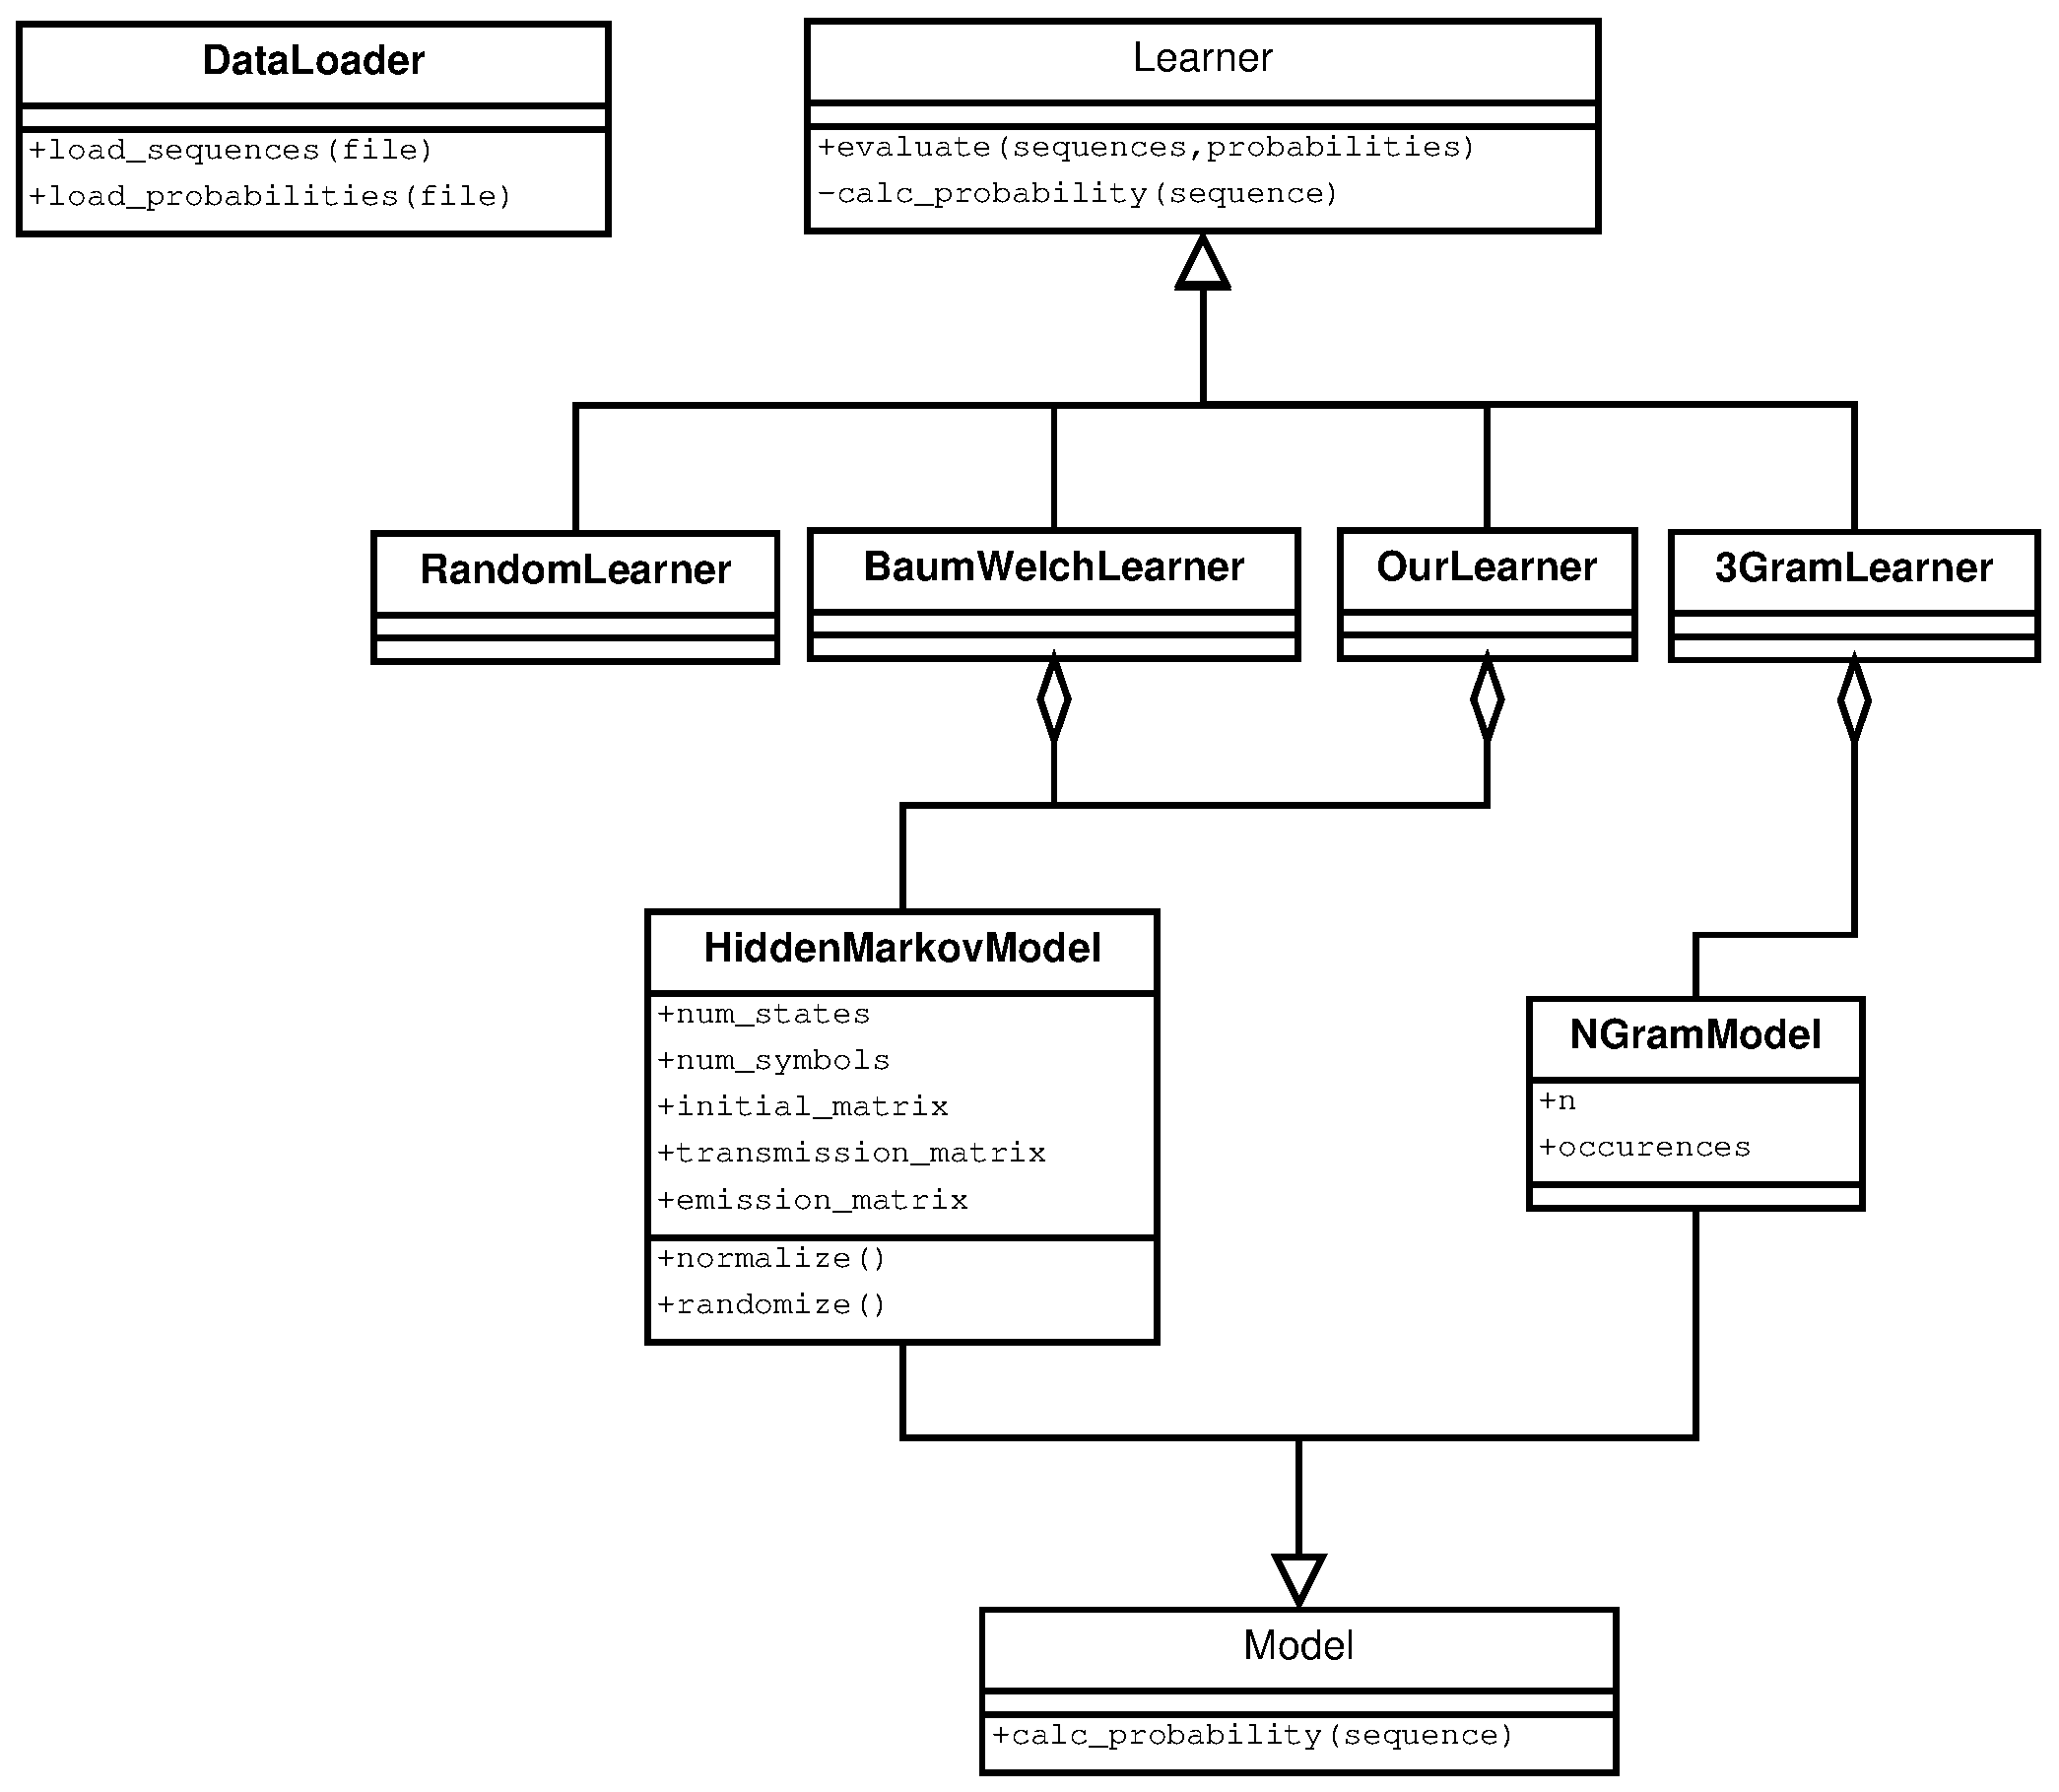
\includegraphics[scale=.4]{pictures/test-environment-overview.eps}
\caption{An overview of the test environment}
\label{fig:testenvironment}
\end{figure}

